% Provenance (never printed): see sources/outline_sources.md (Year 3: rift
% models, normal-fault systems, metamorphic core complexes, strike-slip
% systems). Brief: sources/book5/BRIEFS.md, ch. 9. Curves from
% figdata/bachelor-3/domino_extension.py and rollover.py. Exercise and problem
% values in the Book 5 scratch calculator calc/ch09.py.
\chapter{प्रसारी और स्ट्राइक-स्लिप विवर्तनिकी}\label{ch:b3:extension-strike-slip}

सिएरा नेवादा और कोलोराडो पठार के बीच परास और द्रोणियाँ
किसी खेत की नालियों की तरह एक के बाद एक आती हैं, हर परास भूपर्पटी का
एक सामान्य भ्रंश के साथ झुका हुआ खंड है। इन परासों में से कुछ के क्रोड में वे चट्टानें,
जो 23 से \qty{30}{km} गहराई तक और 500 से \qty{650}{\celsius} तापमान पर दबी थीं, अब
सतह पर आ गई हैं, केवल कुछ अंश की नति वाले एक ही भ्रंश के नीचे। एक महाद्वीप
दो गुणक से खींचकर अलग किया जा सकता है, और उन भ्रंशों के साथ पार्श्व में फाड़ा जा सकता है
जो मुड़ते हैं, सीढ़ीनुमा होते हैं और \qty{10}{km} तक गहरी द्रोणियाँ खोलते हैं। यह अध्याय
प्रसार और स्ट्राइक-स्लिप भ्रंशन की ज्यामिति, उसे नियंत्रित करने वाले कुछ नियम
और वास्तविक तंत्र जो साक्ष्य छोड़ते हैं, उन्हें विकसित करता है।
% ledger: cooper10:snake-range, mcq05:basin-range, tb93:dead-sea-basin

\begin{recall}
सामान्य, स्ट्राइक-स्लिप और रूपांतर भ्रंश, अर्ध-ग्राबेन और महाद्वीपीय
दरार पुस्तक 3 (स्नातक वर्ष 1) में हैं, उसके दरार, भ्रंश, वलन और विन्यास वाले अध्यायों में,
और एंडरसन के सिद्धांत के साथ: जब $\sigma_1$ ऊर्ध्वाधर हो, तो सामान्य भ्रंशों की
नति $\ang{45} + \phi/2$, यानी लगभग \ang{60} होती है; जब $\sigma_2$ ऊर्ध्वाधर हो, तो स्ट्राइक-स्लिप
भ्रंश $\ang{45} - \phi/2$ कोण पर स्ट्राइक करते हैं, जो $\sigma_1$ से मापा जाता है। चट्टान-घर्षण का
बायरली नियम, $\tau = 0.85\,\sigma_n$ \qty{200}{MPa} से नीचे और $\tau =
\qty{50}{MPa} + 0.6\,\sigma_n$ ऊपर, प्रतिबल, विकृति
और प्रवाहिकी वाले अध्याय में है। खिंचाव प्रतिरूप, जिसमें स्थलमंडल समान रूप से
गुणक $\beta$ से पतला होता है, और दरार-द्रोणी पुस्तक 4 (स्नातक वर्ष 2) में हैं, उसके
अवसादी द्रोणियों की तुलना वाले अध्याय में। \omterm{def:b3:deformation-mechanisms:shear-zone}{अपरूपण क्षेत्र} और मायलोनाइट
\cref{ch:b3:deformation-mechanisms} में हैं; विलगन तक की गहराई अतिरिक्त क्षेत्रफल
$A = Sh$ से, \cref{ch:b3:structural-analysis} में।
\end{recall}
% ledger: byerlee:1975

\section{दरार के दो प्रतिरूप}\label{sec:b3:extension-strike-slip:models}

पुस्तक 4 (स्नातक वर्ष 2) का खिंचाव प्रतिरूप पूरे स्थलमंडल को उसी जगह के नीचे
एक ही गुणक से पतला करता है: भूपर्पटी और प्रावार साथ-साथ पतले होते हैं,
सममित रूप से, शुद्ध कर्तन द्वारा। कई दरारी किनारे सममित नहीं होते: एक ओर
झुके हुए खंडों का चौड़ा क्षेत्र है, दूसरी ओर संकरी खड़ी ढलान, और
प्रावार का पतलापन भूपर्पटी के पतलेपन के नीचे नहीं, बल्कि उसके बगल में पड़ता है।

\begin{definition}[सरल-अपरूपण दरार मॉडल]\label{def:b3:extension-strike-slip:rift-models}
\emph{सरल-अपरूपण दरार मॉडल}\index{सरल-अपरूपण दरार मॉडल} में स्थलमंडल
एक निम्न-कोण \omterm{def:b3:deformation-mechanisms:shear-zone}{अपरूपण क्षेत्र} के साथ अलग खींचा जाता है, जो उसे
सतह से उसके तल तक काटता है। \omterm{def:b3:deformation-mechanisms:shear-zone}{अपरूपण क्षेत्र} के ऊपर की प्लेट, यानी ऊपरी प्लेट, अपना निचला
भाग खो देती है; नीचे की प्लेट, यानी निचली प्लेट, उसके नीचे से बाहर खींची जाती है।
नीचे से बाहर खींची जाती है। भूपर्पटी का पतलापन और प्रावार का पतलापन पार्श्व में
एक-दूसरे से विस्थापित होते हैं, और जब महाद्वीप टूटता है तो बनने वाले दोनों युग्मी
किनारे असममित होते हैं।
\end{definition}

वास्तविक दरारों में दोनों मिले होते हैं: ऊपरी भूपर्पटी में भंगुर भ्रंशन, तन्य पतलापन
नीचे, और एक ऐसा प्रावार जो भूपर्पटी से चौड़े या संकरे क्षेत्र में पतला हो सकता है
(गहराई-निर्भर खिंचाव)। जहाँ तप्त प्रावार दरार के नीचे ऊपर उठता है, या
सरल-अपरूपण स्थिति में उसके पार्श्व के नीचे, वहाँ उत्प्लावकता दरार के कंधों को उठाती है,
जो द्रोणी के तल से ऊपर पर्वतों के रूप में खड़े रहते हैं।

\begin{omfigure}
\begin{tikzpicture}[scale=0.95, >=stealth]
% (क) pure shear
\begin{scope}
\fill[omLithBasalt!40] (0,-3.2) rectangle (6.6,-1.3);
\fill[omLithGranite!50] (0,0) -- (2.2,0) -- (2.5,-0.35) -- (4.1,-0.35) -- (4.4,0) -- (6.6,0) -- (6.6,-1.3)
  -- (4.4,-1.3) -- (3.3,-0.95) -- (2.2,-1.3) -- (0,-1.3) -- cycle;
\fill[omLithBasalt!40] (2.2,-1.3) -- (3.3,-0.95) -- (4.4,-1.3) -- cycle;
\fill[orange!25] (0,-3.2) -- (1.8,-3.2) -- (3.3,-2.1) -- (4.8,-3.2) -- (6.6,-3.2) -- (6.6,-3.7) -- (0,-3.7) -- cycle;
\draw (0,0) -- (2.2,0) -- (2.5,-0.35) -- (4.1,-0.35) -- (4.4,0) -- (6.6,0);
\draw (0,-1.3) -- (2.2,-1.3) -- (3.3,-0.95) -- (4.4,-1.3) -- (6.6,-1.3);
\draw (0,-3.2) -- (1.8,-3.2) -- (3.3,-2.1) -- (4.8,-3.2) -- (6.6,-3.2);
\draw[thick] (2.2,0) -- (2.75,-0.85); \draw[thick] (4.4,0) -- (3.85,-0.85);
\node[font=\scriptsize] at (0.7,-0.65) {भूपर्पटी};
\node[font=\scriptsize, align=center] at (0.9,-2.25) {प्रावार\\ स्थलमंडल};
\node[font=\scriptsize] at (1.2,-3.48) {दुर्बलमंडल};
\draw[<-] (-0.1,0.25) -- (0.6,0.25); \draw[->] (6.0,0.25) -- (6.7,0.25);
\node[font=\small] at (3.3,-4.2) {(क) शुद्ध कर्तन};
\end{scope}
% (ख) simple shear: crust thinned near the breakaway (left), mantle beneath the upper plate (right)
\begin{scope}[xshift=7.4cm]
\fill[omLithBasalt!40] (0,-3.2) rectangle (6.6,-1.3);
\fill[omLithGranite!50] (0,0) -- (0.9,0) -- (1.2,-0.3) -- (2.2,-0.3) -- (2.5,0) -- (4.0,0)
  .. controls (4.6,0.18) and (5.2,0.18) .. (5.8,0) -- (6.6,0) -- (6.6,-1.3)
  -- (2.9,-1.3) -- (2.0,-0.7) -- (1.2,-1.3) -- (0,-1.3) -- cycle;
\fill[omLithBasalt!40] (1.2,-1.3) -- (2.0,-0.7) -- (2.9,-1.3) -- cycle;
\fill[orange!25] (0,-3.2) -- (3.4,-3.2) -- (4.8,-2.1) -- (6.0,-3.2) -- (6.6,-3.2) -- (6.6,-3.7) -- (0,-3.7) -- cycle;
\draw (0,0) -- (0.9,0) -- (1.2,-0.3) -- (2.2,-0.3) -- (2.5,0) -- (4.0,0)
  .. controls (4.6,0.18) and (5.2,0.18) .. (5.8,0) -- (6.6,0);
\draw (0,-1.3) -- (1.2,-1.3) -- (2.0,-0.7) -- (2.9,-1.3) -- (6.6,-1.3);
\draw (0,-3.2) -- (3.4,-3.2) -- (4.8,-2.1) -- (6.0,-3.2) -- (6.6,-3.2);
\draw[omThm, very thick] (0.9,0) .. controls (2.4,-0.9) and (3.9,-1.8) .. (5.4,-3.2);
\node[font=\scriptsize, align=center] at (5.0,-0.6) {ऊपरी प्लेट};
\node[font=\scriptsize, align=center] at (1.3,-2.3) {निचली प्लेट};
\node[omThm, font=\scriptsize, align=center] at (3.0,-2.15) {अपरूपण\\ क्षेत्र};
\node[font=\scriptsize, align=center] at (4.9,0.42) {उत्थित पार्श्व};
\draw[<-] (-0.1,0.25) -- (0.6,0.25); \draw[->] (6.0,0.25) -- (6.7,0.25);
\node[font=\small] at (3.3,-4.2) {(ख) सरल कर्तन};
\end{scope}
\end{tikzpicture}

\par\smallskip{\small दरार के दो चरम प्रतिरूप (पैमाने पर नहीं)। (क) शुद्ध
कर्तन: भूपर्पटी और प्रावार-स्थलमंडल दरार के नीचे साथ-साथ पतले होते हैं, दोनों ओर
सामान्य भ्रंशों के साथ। (ख) सरल कर्तन: एक निम्न-कोण \omterm{def:b3:deformation-mechanisms:shear-zone}{अपरूपण क्षेत्र}
स्थलमंडल को पार करता है; भूपर्पटी अपने सतही निशान के पास पतली होती है, प्रावार
दूरवर्ती ओर, ऊपरी प्लेट के नीचे, पतला होता है, इसलिए दरार असममित होती है और
उसके पतले प्रावार के ऊपर का पार्श्व उत्थित होता है।}\label{fig:b3:extension-strike-slip:models}
\end{omfigure}

\section{सामान्य-भ्रंश तंत्र}\label{sec:b3:extension-strike-slip:faults}

\begin{definition}[डोमिनो भ्रंशन]\label{def:b3:extension-strike-slip:domino}
\emph{डोमिनो भ्रंशन}\index{डोमिनो भ्रंशन} में समांतर समतलीय सामान्य भ्रंशों का एक समुच्चय ऊपरी भूपर्पटी को
कठोर खंडों में बाँट देता है, जो क्षेत्र के फैलने के साथ किताबों की
पंक्ति के गिरने की तरह एक साथ घूमते हैं: भ्रंश कम खड़े होते जाते हैं और
संस्तर, जो पहले क्षैतिज थे, दूसरी दिशा में झुक जाते हैं।
\end{definition}

\begin{theorem}[डोमिनो द्वारा प्रसार]\label{thm:b3:extension-strike-slip:domino}
मान लीजिए समांतर समतलीय भ्रंशों से घिरे कठोर खंड, जिनके भ्रंश पहले $\theta_0$ नति पर थे,
तब तक घूमें जब तक भ्रंश $\theta$ नति न ले लें। फिर संस्तर भ्रंशों से दूर की ओर $\theta_0
- \theta$ नति से झुकते हैं, और क्षेत्र
गुणक से विस्तारित हुआ है:
\[
  \beta = \frac{\sin\theta_0}{\sin\theta} .
\]
\end{theorem}

\begin{proof}
खंड कठोर हैं, इसलिए दो निकटवर्ती भ्रंशों के बीच की लंबवत दूरी $d$
नहीं बदलती। क्षैतिज रेखा के अनुदिश दो समांतर
समतल, जो $\theta$ नति पर हैं और $d$ दूरी पर हैं, लंबाई $d/\sin
\theta$ का एक खंड काटते हैं; क्षेत्र की चौड़ाई उस खंड की लंबाई के अनुपात में बदलती है,
$d/\sin\theta_0$ से $d/\sin\theta$ तक। खंड उस कोण से घूमते हैं जिससे भ्रंश चपटे हुए हैं,
अर्थात् $\theta_0 - \theta$, और संस्तर, जो पहले क्षैतिज थे,
उनके साथ घूमते हैं।
\end{proof}

केवल घूर्णन से सीमित विस्तार मिलता है: जो भ्रंश \ang{60} नति पर आरंभ होते हैं और
\ang{30} तक चपटे होते हैं, तो क्षेत्र $\beta = 1.73$ गुणक से विस्तारित होता है। वे
सदा के लिए नहीं घूम सकते: भ्रंश जितना चपटा होता है, उसका सरकना उतना ही कठिन होता जाता है, क्योंकि ऊर्ध्वाधर
$\sigma_1$ उस पर अधिक दबाव डालता है और उसे कम अपरूपित करता है।

\begin{proposition}[सामान्य भ्रंश का घर्षणी लॉक-अप]\label{prop:b3:extension-strike-slip:lockup}
मान लीजिए घर्षण गुणांक $\mu$ वाला एक संसंजनहीन भ्रंश
$t$ कोण बनाता है $\sigma_1$ से, सभी प्रतिबल प्रभावी हैं। यह तब सरकता है जब
मुख्य प्रतिबलों का अनुपात इस मान तक पहुँचता है:
\[
  \frac{\sigma_1}{\sigma_3} = \frac{1 + \mu\cot t}{1 - \mu\tan t} ,
\]
यह न्यूनतम है, $(\sqrt{1 + \mu^2} + \mu)^2$, जब $\tan2t = 1/\mu$ है, और
अनंत है जब $\tan t = 1/\mu$ है। $\sigma_1$ ऊर्ध्वाधर होने पर भ्रंश की नति
$\ang{90} - t$ होती है: $\arctan\mu$ से कम नति वाला सामान्य भ्रंश
बिल्कुल नहीं सरक सकता।
\end{proposition}

\begin{proof}
मान लीजिए $m = (\sigma_1 + \sigma_3)/2$ और $s = (\sigma_1 - \sigma_3)/2$। समतल पर
$\sigma_n = \sigma_1\sin^2t + \sigma_3\cos^2t = m - s\cos2t$ और
$\tau = (\sigma_1 - \sigma_3)\sin t\cos t = s\sin2t$। सरकने के लिए शर्त है $\tau =
\mu\sigma_n$; $\sigma_3\sin t\cos t$ से भाग देने और $\sigma_1$ को एकत्र करने पर
अनुपात प्राप्त होता है, जिसका हर $\tan t = 1/\mu$ पर शून्य हो जाता है। दूसरे रूप में
रूप में प्रतिबंध इस प्रकार है $s(\sin2t + \mu\cos2t) = \mu m$। कोष्ठक का मान
अधिक से अधिक $\sqrt{1 + \mu^2}$ होता है, जो $\tan2t = 1/\mu$ पर प्राप्त होता है, जहाँ सरकने के लिए
न्यूनतम $s/m = \mu/\sqrt{1 + \mu^2}$ चाहिए; तब $\sigma_1/\sigma_3 = (m + s)/(m - s) =
(\sqrt{1 + \mu^2} + \mu)/(\sqrt{1 + \mu^2} - \mu) = (\sqrt{1 + \mu^2} +
\mu)^2$, क्योंकि अंतिम दो कोष्ठकों का गुणनफल 1 है।
\end{proof}

बायरली के $\mu = 0.6$ के लिए, सबसे उपयुक्त दिशा वाला सामान्य भ्रंश \ang{60.5} नति पर है और
तब सरकता है जब $\sigma_1 = 3.12\,\sigma_3$ हो; \ang{45} नति पर स्थित भ्रंश के लिए $4.0$ चाहिए, और
\ang{31} से कम नति वाला कोई भी नहीं सरकता; $\mu = 0.85$ के साथ लॉक-अप नति
\ang{40} है। नीचे दिया गया चित्र दोनों परिणाम दिखाता है। जब डोमिनो का एक समुच्चय
लॉक-अप के निकट पहुँचता है, तो एक नया तीव्र भ्रंश समुच्चय पुराने को काटता है: अत्यधिक विस्तारित क्षेत्र
भ्रंशों की कई पीढ़ियाँ दिखाते हैं।

\begin{omfigure}
\begin{tikzpicture}
\begin{groupplot}[group style={group size=2 by 1, horizontal sep=1.6cm},
  omrecord, width=0.47\linewidth, height=0.42\linewidth, title style={font=\small},
  legend style={font=\scriptsize, legend cell align=left}]
\nextgroupplot[title={(क) कठोर डोमिनो द्वारा विस्तार}, xlabel={वर्तमान भ्रंश नति $\theta$ (\unit{\degree})},
  ylabel={विस्तार गुणक $\beta$}, xmin=10, xmax=70, ymin=1, ymax=4,
  legend style={at={(0.97,0.97)}, anchor=north east}]
% computed in figdata/bachelor-3/domino_extension.py
\addplot[omDef, thick] table[x=dip, y=b70] {figdata/out/bachelor-3-domino_extension-beta.dat};
\addlegendentry{$\theta_0 = \ang{70}$}
\addplot[red!70!black, thick, densely dashed] table[x=dip, y=b60] {figdata/out/bachelor-3-domino_extension-beta.dat};
\addlegendentry{$\theta_0 = \ang{60}$}
\addplot[black, thick, densely dotted] table[x=dip, y=b45] {figdata/out/bachelor-3-domino_extension-beta.dat};
\addlegendentry{$\theta_0 = \ang{45}$}
\nextgroupplot[title={(ख) सरकने हेतु प्रतिबल अनुपात}, xlabel={भ्रंश नति (\unit{\degree})},
  ylabel={$\sigma_1/\sigma_3$}, xmin=20, xmax=90, ymode=log, ymin=1, ymax=40,
  log ticks with fixed point, ytick={1,2,5,10,20,40},
  legend style={at={(0.97,0.97)}, anchor=north east}]
\addplot[omDef, thick] table[x=dip, y=r060] {figdata/out/bachelor-3-domino_extension-lockup.dat};
\addlegendentry{$\mu = 0.6$}
\addplot[red!70!black, thick, densely dashed] table[x=dip, y=r085] {figdata/out/bachelor-3-domino_extension-lockup.dat};
\addlegendentry{$\mu = 0.85$}
\end{groupplot}
\end{tikzpicture}

\par\smallskip{\small (क) कठोर डोमिनो के क्षेत्र का विस्तार गुणक, जब उसके भ्रंश
प्रारंभिक नति $\theta_0$ से $\theta$ तक घूमते हैं। (ख) दी गई नति वाले सामान्य भ्रंश को
सरकाने के लिए आवश्यक प्रभावी मुख्य प्रतिबलों का अनुपात, जब
ऊर्ध्वाधर $\sigma_1$ के अंतर्गत, बायरली के दो घर्षण गुणांकों के लिए: न्यूनतम
\ang{60} और \ang{65} के निकट, और लॉक-अप नतियों \ang{31} और
\ang{40} पर अनंत।}\label{fig:b3:extension-strike-slip:domino}
\end{omfigure}

कई बड़े सामान्य भ्रंश वक्राकार होते हैं, जो सतह पर तीव्र होते हैं और
गहराई पर लगभग क्षैतिज भ्रंश या \omterm{def:b3:deformation-mechanisms:shear-zone}{अपरूपण क्षेत्र} में चपटे हो जाते हैं।

\begin{definition}[विलगन भ्रंश, लिस्ट्रिक भ्रंश, रोलओवर अपनति]\label{def:b3:extension-strike-slip:detachment}
\emph{विलगन भ्रंश}\index{विलगन भ्रंश} एक निम्न-कोण सामान्य भ्रंश
या \omterm{def:b3:deformation-mechanisms:shear-zone}{अपरूपण क्षेत्र} है, जिसका विस्थापन बड़ा होता है, किलोमीटर से दसियों किलोमीटर तक, जो
एक विस्तारित ऊपरी प्लेट को भिन्न रूप से विरूपित निचली प्लेट से अलग करता है।
\emph{लिस्ट्रिक भ्रंश}\index{लिस्ट्रिक भ्रंश} वह सामान्य भ्रंश है जिसकी नति
गहराई के साथ घटती है, इसकी रूपरेखा ऊपर की ओर अवतल होती है। लिस्ट्रिक भ्रंश की
ऊपरी भित्ति नीचे और दूर खिसकती है, तो वह भ्रंश के साथ संपर्क बनाए रखने के लिए मुड़ती है:
इसके संस्तर एक चौड़े वलन में भ्रंश की ओर झुकते हैं, जिसे \emph{रोलओवर
अपनति}\index{रोलओवर अपनति} कहते हैं।
\end{definition}

\begin{method}[स्थिर क्षैतिज विस्थापन की रचना]\label{met:b3:extension-strike-slip:heave}
\omterm{def:b3:extension-strike-slip:detachment}{लिस्ट्रिक भ्रंश} की ऊपरी भित्ति को एक क्षैतिज विस्थापन के बाद खींचने के लिए
$H$, अर्थात् क्षैतिज विस्थापन, सरकन की दिशा के समांतर एक परिच्छेद पर:
\begin{enumerate}
  \item ऊपरी भित्ति को ऊर्ध्वाधर स्तंभों में बाँटिए। प्रत्येक स्तंभ को
        निचली भित्ति से दूर की ओर $H$ के बराबर बगल में खिसकाइए।
  \item प्रत्येक स्तंभ को उसके नीचे के भ्रंश के गिराव जितना नीचे लाइए: वह स्तंभ, जो
        जहाँ भ्रंश गहराई $f(x)$ पर है, वहाँ से शुरू होता है और जहाँ वह
        $f(x + H)$ पर है वहाँ समाप्त होता है, वह $f(x + H) - f(x)$ नीचे गिरता है, जिससे उसका आधार
        भ्रंश पर वापस आ जाए।
  \item निचली भित्ति और खिसकी हुई ऊपरी भित्ति के बीच बची जगह अर्ध-ग्राबेन है, जो
        खुलते समय उन अवसादों से भरता है जो भ्रंश की ओर
        मोटे होते जाते हैं।
\end{enumerate}
पीछे की ओर पढ़ने पर यह रचना परिच्छेद को पुनर्स्थापित करती है और
रोलओवर के आकार से भ्रंश के आकार का पूर्वानुमान लगाती है।
\end{method}

भ्रंश से गिने गए, किसी संस्तर के मूल स्तर के नीचे का क्षेत्रफल
\cref{ch:b3:structural-analysis} में दिए क्षेत्रफल का चिह्न बदला हुआ रूप है: $A =
H(D - z_0)$ उस संस्तर के लिए, जो $z_0$ गहराई पर पहले विलगन के ऊपर है, जिसकी
गहराई $D$ है, क्योंकि संस्तर के नीचे की चट्टान अपना क्षेत्रफल बनाए रखती है, जबकि उसकी लंबाई
$H$ से बढ़ती है। भूकंपीय खंड पर $A$ और $H$ मापने से विलगन की गहराई मिलती है।
नीचे की आकृति इस रचना को दर्शाती है।

\begin{omfigure}
\begin{tikzpicture}
\begin{axis}[width=0.9\linewidth, height=0.36\linewidth, omsection,
  xmin=-2, xmax=24, ymin=0, ymax=6, y dir=reverse,
  xlabel={दूरी (\unit{km})}, ylabel={गहराई (\unit{km})},
  legend style={font=\scriptsize, legend cell align=left, at={(0.98,0.27)}, anchor=south east}]
% computed in figdata/bachelor-3/rollover.py (heave 2 km, detachment at 5 km)
\addplot[name path=fault, black, very thick] table[x=x, y=z] {figdata/out/bachelor-3-rollover-fault.dat};
\addlegendentry{लिस्ट्रिक भ्रंश}
\addplot[name path=top, omDef, thick] table[x=x, y=z] {figdata/out/bachelor-3-rollover-top.dat};
\addlegendentry{ऊपरी भित्ति का शीर्ष}
\addplot[omDef, thick, densely dashed] table[x=x, y=z] {figdata/out/bachelor-3-rollover-bed.dat};
\addlegendentry{पहले \qty{2}{km} पर स्थित एक संस्तर}
\addplot[gray, dashed, forget plot] coordinates {(-2,0) (24,0)};
\addplot[gray, dashed, forget plot] coordinates {(-2,5) (24,5)};
\node[font=\scriptsize, anchor=west] at (axis cs:15,5.35) {विलगन};
\node[font=\scriptsize] at (axis cs:3.9,0.45) {अर्ध-ग्राबेन};
\node[font=\scriptsize] at (axis cs:-1,1.5) {निचली भित्ति};
\node[font=\scriptsize] at (axis cs:9.5,1.15) {रोलओवर};
\end{axis}
\end{tikzpicture}

\par\smallskip{\small सतह पर \ang{60} पर नत एक \omterm{def:b3:extension-strike-slip:detachment}{लिस्ट्रिक भ्रंश}, जो
\qty{5}{km} पर एक विलगन में समतल होता है, और \qty{2}{km} का क्षैतिज विस्थापन,
स्थिर-विस्थापन रचना से खींचा गया है। ऊपरी भित्ति का शीर्ष और एक गहरा संस्तर
भ्रंश की ओर धँसकर एक रोलओवर बनाते हैं; मूल
शीर्ष के नीचे का क्षेत्रफल, \qty{10}{km^2}, विस्थापन और विलगन की गहराई का गुणनफल है, और गहरे संस्तर के नीचे का
क्षेत्रफल \qty{6}{km^2} है, जो उसके ऊपर की ऊँचाई और विस्थापन का गुणनफल है।}\label{fig:b3:extension-strike-slip:rollover}
\end{omfigure}

सामान्य भ्रंश अनंत नहीं होते। जहाँ एक भ्रंश स्ट्राइक के अनुदिश लुप्त होता है, उसका
विस्थापन दूसरे भ्रंश में चला जाता है, जो प्रायः विपरीत दिशा में नत होता है, और दरार के
अर्ध-ग्राबेन उसकी लंबाई के साथ ध्रुवता में एकांतरित होते हैं।

\begin{definition}[स्थानांतरण क्षेत्र]\label{def:b3:extension-strike-slip:transfer}
\emph{स्थानांतरण क्षेत्र}\index{स्थानांतरण क्षेत्र} वह क्षेत्र है, जो दो
अतिव्यापी या विस्थापित सामान्य-भ्रंश खंडों, या दरार-खंडों के बीच स्थित है और जिसके आर-पार प्रसार
एक से दूसरे तक जाता है: समान ध्रुवता के दो भ्रंशों के बीच एक रिले रैंप,
विपरीत ध्रुवता के अर्ध-ग्राबेनों के बीच एक उच्चभूमि, या
प्रसार के समांतर एक स्ट्राइक-स्लिप भ्रंश, यानी स्थानांतरण भ्रंश।
\end{definition}

\section{कायांतरी क्रोड संकुल}\label{sec:b3:extension-strike-slip:core}

\begin{definition}[कायांतरी क्रोड संकुल, लुढ़कता मोड़]\label{def:b3:extension-strike-slip:core-complex}
\emph{कायांतरी क्रोड संकुल}\index{कायांतरी क्रोड संकुल} मध्य या निचली भूपर्पटी से ऊपर लाई गई
कायांतरित चट्टानों और मायलोनाइटों का एक गुंबद है, जो एक \omterm{def:b3:extension-strike-slip:detachment}{विलगन भ्रंश} के नीचे स्थित है,
जिसकी ऊपरी प्लेट ऊपरी भूपर्पटी की चट्टानों के झुके हुए खंडों का मोज़ेक है।
\emph{लुढ़कता मोड़}\index{लुढ़कता मोड़} मॉडल में विलगन गहराई पर मध्यम नति पर फिसलता है; जैसे-जैसे ऊपरी प्लेट दूर खिसकती है,
भारमुक्त निचली भित्ति समस्थिति से ऊपर उठती है और मुड़ती है, इसलिए
भ्रंश का हर भाग निम्न नति तक घूम जाता है और फिसलना बंद कर देता है,
जब वह एक ऐसे मोड़ से गुज़र जाता है
जो प्रसार के साथ खिसकता है।
\end{definition}

निचली भित्ति के मायलोनाइट कहानी के गहरे भाग का अभिलेख रखते हैं: ये
\cref{ch:b3:deformation-mechanisms} में वर्णित \omterm{def:b3:deformation-mechanisms:shear-zone}{अपरूपण क्षेत्र} हैं, और उनके
\omterm{def:b3:deformation-mechanisms:kinematic}{शुद्धगतिक सूचक} ऊपरी प्लेट के विस्थापन की दिशा बताते हैं। ऊपर की ओर वही
चट्टानें भंगुर--तन्य संक्रमण से गुज़रती हैं और भ्रंश के ठीक नीचे
कैटाक्लासाइट और ब्रेक्सिया से अधिलेखित हो जाती हैं। नेवादा की उत्तरी स्नेक रेंज में,
निचली भित्ति के गार्नेट-युक्त शिस्ट 6 से \qty{8}{kbar} दाब और
500 से \qty{650}{\celsius} तापमान तक पहुँचे; दफ़न गहराई 23 से \qty{30}{km} थी;
उन्हें ऊपर लाने वाला विलगन \omterm{def:b3:extension-strike-slip:core-complex}{लुढ़कता मोड़} समझा जाता है।
% ledger: cooper10:snake-range

\begin{omfigure}
\begin{tikzpicture}[scale=1.0, >=stealth]
% upper plate dominoes on the left
\foreach \x in {0.0,0.9,1.8} {
  \fill[omLithSand] (\x,0) -- (\x+0.8,0) -- (\x+1.3,-0.9+0.25*\x) -- (\x+0.4,-1.5+0.2*\x) -- cycle;
  \draw (\x,0) -- (\x+0.8,0) -- (\x+1.3,-0.9+0.25*\x) -- (\x+0.4,-1.5+0.2*\x) -- cycle;
}
\fill[omLithGranite!45] (0,-2.6) -- (0,-1.6) .. controls (2.5,-1.2) and (4.0,-0.15) .. (6.0,-0.1)
  .. controls (8.0,-0.15) and (9.5,-0.9) .. (11.2,-1.0) -- (11.2,-2.6) -- cycle;
\fill[pattern=horizontal lines, pattern color=gray] (0,-1.6) .. controls (2.5,-1.2) and (4.0,-0.15) .. (6.0,-0.1)
  .. controls (8.0,-0.15) and (9.5,-0.9) .. (11.2,-1.0) -- (11.2,-1.35)
  .. controls (9.5,-1.25) and (8.0,-0.5) .. (6.0,-0.45) .. controls (4.0,-0.5) and (2.5,-1.55) .. (0,-1.95) -- cycle;
\draw[omThm, very thick] (0,-1.6) .. controls (2.5,-1.2) and (4.0,-0.15) .. (6.0,-0.1)
  .. controls (8.0,-0.15) and (9.5,-0.9) .. (11.2,-1.0);
% upper plate to the right, still in place
\fill[omLithSand] (8.4,0) -- (11.2,0) -- (11.2,-1.0) .. controls (10.2,-0.95) and (9.3,-0.75) .. (8.4,-0.35) -- cycle;
\draw (8.4,0) -- (11.2,0); \draw (8.4,0) -- (8.4,-0.35);
\node[font=\scriptsize] at (9.9,-0.45) {ऊपरी प्लेट};
\node[font=\scriptsize] at (1.5,0.3) {झुके हुए खंड};
\node[omThm, font=\scriptsize] at (6.0,0.15) {विलगन};
\node[font=\scriptsize] at (6.0,-0.75) {मायलोनाइट};
\node[font=\scriptsize, align=center] at (6.0,-1.8) {मध्य-भूपर्पटी\\ निचली भित्ति};
\draw[->, thick] (6.0,-2.9) -- (6.0,-2.2) node[pos=0, below, font=\scriptsize] {समस्थितिक उत्थान};
\draw[->, omThm] (10.4,0.3) -- (11.1,0.3);
\draw[->, omThm] (1.0,0.55) -- (0.3,0.55);
\draw[dashed] (7.6,-0.3) -- (8.6,-1.5) node[below, font=\scriptsize] {लुढ़कता मोड़};
\end{tikzpicture}

\par\smallskip{\small \omterm{def:b3:extension-strike-slip:core-complex}{कायांतरी क्रोड संकुल} की संरचना (पैमाने पर नहीं)।
विलगन की निचली भित्ति, मध्य-भूपर्पटी की चट्टानों का एक गुंबद है, जिसके ऊपर
मायलोनाइटों का कवच है; यह ऊपरी प्लेट के दोनों ओर खिंचने पर उसके नीचे
ऊपर उठता है। विलगन का वह भाग, जो \omterm{def:b3:extension-strike-slip:core-complex}{लुढ़कता मोड़} पार कर चुका है,
निम्न नति तक मुड़ गया है और अब नहीं फिसलता। ऊपरी प्लेट के झुके हुए खंड
विलगन पर टिके हैं।}\label{fig:b3:extension-strike-slip:core}
\end{omfigure}

निम्न नतियाँ एक विरोधाभास हैं: लॉक-अप प्रतिज्ञप्ति के अनुसार कोई सामान्य भ्रंश, जिसकी
नति लगभग \ang{31} से कम हो, बायरली घर्षण के साथ ऊर्ध्वाधर $\sigma_1$ के अंतर्गत फिसलना नहीं चाहिए।
\omterm{def:b3:extension-strike-slip:core-complex}{लुढ़कता मोड़} इससे निकलने का एक रास्ता है: भ्रंश का सक्रिय भाग
जितना देखा गया है उससे अधिक नत है। अन्य कारण हैं मिट्टियों से दुर्बल हुआ भ्रंश
या उच्च दाब पर तरलों से दुर्बल हुआ भ्रंश, जो प्रभावी $\mu$ घटाता है, या प्रतिबल
क्षेत्र, जो गहराई पर एक \omterm{def:b3:deformation-mechanisms:shear-zone}{अपरूपण क्षेत्र} के पास घूर्णित है; निम्न-कोण सामान्य भ्रंशों पर भूकंप
दुर्लभ हैं, जो तीव्र नति पर फिसलने, या बिना भूकंप के फिसलने के पक्ष में है।

\section{स्ट्राइक-स्लिप तंत्र}\label{sec:b3:extension-strike-slip:strike-slip}

मिट्टी-केक प्रयोगों में और प्रकृति में, स्ट्राइक-स्लिप भ्रंश अवसादों के आवरण में
कोई साफ़ तल नहीं काटता: वह छोटे, एक-दूसरे से हटे हुए विभंगों की एक पट्टी के रूप में बढ़ता है,
जिनके कोण एकसमान होते हैं।

\begin{definition}[रीडेल अपरूपण]\label{def:b3:extension-strike-slip:riedel}
स्ट्राइक-स्लिप सरल-अपरूपण के एक क्षेत्र में \emph{रीडेल अपरूपण}\index{रीडेल अपरूपण} वे
छोटे अपरूपण विभंग हैं जो सबसे पहले बनते हैं, दो समूहों में: R
अपरूपण, जो क्षेत्र से छोटे कोण पर और उसी विस्थापन-दिशा में होते हैं, तथा R$'$
अपरूपण, जो बड़े कोण पर और विपरीत दिशा में होते हैं। बाद में बनने वाले P अपरूपण, जो क्षेत्र के सापेक्ष R अपरूपणों के सममित होते हैं,
और तनाव-विभंग T इस प्रारूप को पूरा करते हैं।
\end{definition}

\begin{proposition}[रीडेल कोण]\label{prop:b3:extension-strike-slip:riedel}
सरल अपरूपण के एक क्षेत्र में $\sigma_1$ क्षैतिज तल में होता है,
क्षेत्र से \ang{45} पर। कूलॉम्ब कसौटी से टूटने वाली चट्टान के लिए, जिसका आंतरिक घर्षण कोण $\phi$ है,
R \omterm{def:b3:deformation-mechanisms:shear-zone}{अपरूपण क्षेत्र} से $\phi/2$ कोण बनाते हैं, और
R$'$ अपरूपण $\ang{90} - \phi/2$, दोनों क्षेत्र से मापे गए, $\sigma_1$ की ओर वाले पक्ष पर;
तनाव-विभंग $\sigma_1$ के समांतर बनते हैं,
\ang{45} पर।
\end{proposition}

\begin{proof}
सरल अपरूपण में अनंत-सूक्ष्म विकृति की मुख्य दिशाएँ अपरूपण तल से
\ang{45} पर होती हैं, और एक समदैशिक पदार्थ पर $\sigma_1$ उस दिशा में लगता है जिसमें वह सिकुड़ता है।
एंडरसन प्रमेय के अनुसार दोनों कूलॉम्ब तल, जो यहाँ ऊर्ध्वाधर $\sigma_2$ समाहित करते हैं,
$\ang{45} - \phi/2$ कोण बनाते हैं, $\sigma_1$ के दोनों ओर: जो तल क्षेत्र के अधिक निकट है,
वह क्षेत्र से $\ang{45} -
(\ang{45} - \phi/2) = \phi/2$ पर है, और दूसरा $\ang{45} + \ang{45} -
\phi/2$ पर। हर तल इस प्रकार फिसलता है कि $\sigma_1$ के अनुदिश छोटा हो: R \omterm{def:b3:deformation-mechanisms:shear-zone}{अपरूपण क्षेत्र} के साथ,
और R$'$ अपरूपण उसके विरुद्ध। तनाव-विभंग $\sigma_3$ के विरुद्ध खुलते हैं और
उसके लंबवत पड़ते हैं।
\end{proof}

$\phi = \ang{30}$ के लिए R अपरूपण \ang{15} पर स्थित होते हैं, और R$'$ अपरूपण
\ang{75} पर। जहाँ मुख्य भ्रंश सीधा नहीं है, वहाँ उसके दोनों ओर के खंड
उसके आर-पार एक-दूसरे की ओर सिमटते या एक-दूसरे से दूर हटते हैं।

\begin{definition}[अवरोधी मोड़, विमोचक मोड़]\label{def:b3:extension-strike-slip:bends}
स्ट्राइक-स्लिप भ्रंश में मोड़ या सोपान एक \emph{अवरोधी
मोड़}\index{अवरोधी मोड़} होता है जब खंडों की गति उन्हें उसके आर-पार एक-दूसरे की ओर धकेलती है,
और एक \emph{विमोचक मोड़}\index{विमोचक मोड़} जब वह उन्हें अलग खींचती है। दाएँ-पार्श्वीय भ्रंश पर
दाईं ओर का सोपान विमोचक होता है,
और बाईं ओर का अवरोधी; बाएँ-पार्श्वीय भ्रंश के लिए इसका उलटा होता है।
\end{definition}

\begin{definition}[पुल-अपार्ट द्रोणी]\label{def:b3:extension-strike-slip:pull-apart}
एक \emph{पुल-अपार्ट द्रोणी}\index{पुल-अपार्ट द्रोणी} वह द्रोणी है जो दो अतिव्यापी स्ट्राइक-स्लिप
भ्रंश-खंडों के बीच एक विमोचक सोपान पर खुलती है, जिसकी लंबी भुजाएँ इन्हीं खंडों से
और सिरे तिर्यक सामान्य भ्रंशों से सीमित होते हैं।
इसका क्षेत्रफल सोपान की चौड़ाई और भ्रंश के विस्थापन के गुणनफल के समानुपाती बढ़ता है।
\end{definition}

\begin{definition}[पुष्प संरचना]\label{def:b3:extension-strike-slip:flower}
एक \emph{पुष्प संरचना}\index{पुष्प संरचना} भ्रंश-शाखाओं का वह पंखा है जो एक अनुप्रस्थ
काट पर दिखता है, और जिसमें एक तीव्र नति वाला स्ट्राइक-स्लिप भ्रंश सतह के निकट पहुँचते हुए बँट जाता है:
धनात्मक पुष्प, जिसकी शाखाओं में प्रतिलोम घटक होता है और जो एक कटक को उठाता है,
\omterm{def:b3:extension-strike-slip:bends}{अवरोधी मोड़} पर; ऋणात्मक पुष्प, जिसकी शाखाओं में सामान्य घटक होता है
और जो एक अवनमन को घेरता है, \omterm{def:b3:extension-strike-slip:bends}{विमोचक मोड़} पर।
\end{definition}

\begin{definition}[ट्रांसप्रेशन, ट्रांसटेंशन]\label{def:b3:extension-strike-slip:transpression}
\emph{ट्रांसप्रेशन}\index{ट्रांसप्रेशन} वह स्ट्राइक-स्लिप विरूपण है जो क्षेत्र के आर-पार
लघुकरण के साथ मिला हो; \emph{ट्रांसटेंशन}\index{ट्रांसटेंशन} वह स्ट्राइक-स्लिप विरूपण है जो
उसके आर-पार प्रसार के साथ मिला हो। दोनों तब उत्पन्न होते हैं जहाँ दो खंडों के बीच की गति
उनकी सीमा से तिर्यक होती है।
\end{definition}

तिर्यक गति प्रायः विभाजित हो जाती है: एक स्ट्राइक-स्लिप भ्रंश सीमा के समांतर
गति लेता है, और उसके बगल में अधिक्षेप या वलन बनते हैं, या सामान्य भ्रंश
सीमा के आर-पार की गति वहन करते हैं।

\begin{omfigure}
\begin{tikzpicture}[scale=1.0, >=stealth]
% (क) Riedel geometry, dextral E-W zone
\begin{scope}
\draw[thick] (0,0.9) -- (5,0.9); \draw[thick] (0,-0.9) -- (5,-0.9);
\draw[->] (1.0,1.15) -- (2.0,1.15); \draw[->] (4.0,-1.15) -- (3.0,-1.15);
\foreach \x in {0.6,1.6,2.6,3.6} \draw[omDef, thick] (\x,0.2) -- ++(-15:0.9);
\node[omDef, font=\scriptsize] at (4.6,0.05) {R};
\foreach \x in {1.0,2.4} \draw[red!70!black, thick] (\x,-0.6) -- ++(105:0.75);
\node[red!70!black, font=\scriptsize] at (1.0,-0.75) {R$'$};
\foreach \x in {3.3,3.7,4.1} \draw[black, thick] (\x,-0.25) -- ++(15:0.45);
\node[font=\scriptsize] at (4.6,-0.35) {P};
\foreach \x in {0.5,0.9} \draw[omMeth, line width=1.4pt] (\x,0.45) -- ++(135:0.35);
\node[omMeth, font=\scriptsize] at (0.25,0.25) {T};
\draw[<->, omThm] ($(2.6,0)+(135:0.55)$) -- ($(2.6,0)+(-45:0.55)$);
\node[omThm, font=\scriptsize] at (2.05,0.62) {$\sigma_1$};
\node[font=\small] at (2.5,-1.6) {(क) रीडेल अपरूपण, दाएँ-पार्श्वीय};
\end{scope}
% (ख) releasing and restraining steps on a dextral fault
\begin{scope}[xshift=6.0cm]
\fill[omLithSand!70] (1.6,0.75) -- (2.6,0.75) -- (2.6,0.25) -- (1.6,0.25) -- cycle;
\draw[thick] (0,0.75) -- (2.6,0.75); \draw[thick] (1.6,0.25) -- (4.2,0.25);
\draw[->] (0.3,1.0) -- (1.0,1.0); \draw[->] (3.9,0.0) -- (3.2,0.0);
\node[font=\scriptsize] at (2.1,0.5) {द्रोणी};
\node[font=\scriptsize, anchor=west] at (2.75,0.95) {विमोचक};
\fill[omLithGranite!60] (1.6,-0.65) -- (2.6,-0.65) -- (2.6,-1.15) -- (1.6,-1.15) -- cycle;
\draw[thick] (0,-1.15) -- (2.6,-1.15); \draw[thick] (1.6,-0.65) -- (4.2,-0.65);
\draw[->] (0.3,-0.9) -- (1.0,-0.9); \draw[->] (3.9,-0.9) -- (3.2,-0.9);
\node[font=\scriptsize] at (2.1,-0.9) {कटक};
\node[font=\scriptsize, anchor=west] at (2.75,-0.45) {अवरोधी};
\node[font=\small] at (2.1,-1.6) {(ख) सोपान, दाएँ-पार्श्वीय, मानचित्र};
\end{scope}
% (ग) flower structures in section
\begin{scope}[xshift=11.0cm]
\draw[thick] (1.0,-1.3) -- (1.0,-0.4);
\draw[thick] (1.0,-0.4) .. controls (0.9,0.1) .. (0.45,0.8);
\draw[thick] (1.0,-0.4) -- (1.0,0.8);
\draw[thick] (1.0,-0.4) .. controls (1.1,0.1) .. (1.55,0.8);
\draw (0.0,0.8) -- (0.45,0.8) .. controls (0.8,1.1) and (1.2,1.1) .. (1.55,0.8) -- (2.0,0.8);
\node[font=\scriptsize, align=center] at (1.0,-1.6) {धनात्मक};
\draw[thick] (3.2,-1.3) -- (3.2,-0.4);
\draw[thick] (3.2,-0.4) .. controls (3.1,0.1) .. (2.65,0.8);
\draw[thick] (3.2,-0.4) -- (3.2,0.8);
\draw[thick] (3.2,-0.4) .. controls (3.3,0.1) .. (3.75,0.8);
\draw (2.2,0.8) -- (2.65,0.8) .. controls (3.0,0.5) and (3.4,0.5) .. (3.75,0.8) -- (4.2,0.8);
\node[font=\scriptsize, align=center] at (3.2,-1.6) {ऋणात्मक};
\node[font=\small] at (2.1,-1.95) {(ग) पुष्प, अनुप्रस्थ काट};
\end{scope}
\end{tikzpicture}

\par\smallskip{\small स्ट्राइक-स्लिप संरचनाएँ (अनुपात के अनुसार नहीं)। (क) दाएँ-पार्श्वीय
क्षेत्र में, \ang{45} पर $\sigma_1$ के साथ: \ang{15} पर R अपरूपण और
\ang{-15} पर P अपरूपण, दोनों क्षेत्र की दिशा के साथ, R$'$ अपरूपण \ang{75} पर, विपरीत दिशा में,
तनाव दरारें T, $\sigma_1$ के समांतर। (ख) दाएँ-पार्श्वीय भ्रंश पर दाईं ओर का
सोपान एक \omterm{def:b3:extension-strike-slip:pull-apart}{पुल-अपार्ट द्रोणी} खोलता है; बाईं ओर का सोपान एक कटक को ऊपर धकेलता है। (ग) भ्रंश
ऊपर की ओर शाखाओं में बँटकर कटक के नीचे एक धनात्मक पुष्प और अवनमन के नीचे एक ऋणात्मक
पुष्प बनाता है।}\label{fig:b3:extension-strike-slip:strike-slip}
\end{omfigure}

\section{तीन तंत्र}\label{sec:b3:extension-strike-slip:systems}

\paragraph{बेसिन-एंड-रेंज।} इस क्षेत्र का पुनर्निर्माण
\qty{36}{Ma} से लगभग \qty{235}{km} का प्रसार पाया जाता है, जिसकी दिशा
लगभग N\ang{78}W है, उत्तर में, जहाँ यह \qty{50}{\percent} है, और
केंद्र में, जहाँ यह \qty{200}{\percent} तक पहुँचता है: केंद्रीय भाग पहले से तीन गुना चौड़ा हो गया है।
10 से \qty{12}{Ma} पूर्व से, प्रशांत–उत्तर अमेरिका सीमा की दाएँ-पार्श्वीय गति का
एक भाग महाद्वीप में स्थानांतरित हो गया है, लगभग \qty{100}{km} पर, N\ang{25}W दिशा में,
लगभग \qty{1}{cm/yr} की दर से; यह क्षेत्र अब \omterm{def:b3:extension-strike-slip:transpression}{ट्रांसटेंशन} की स्थिति में है।
इसके \omterm{def:b3:extension-strike-slip:core-complex}{कायांतरी क्रोड संकुल} वहाँ स्थित हैं जहाँ प्रसार सबसे अधिक रहा।
% ledger: mcq05:basin-range

\paragraph{मृत सागर।} मृत सागर रूपांतर भ्रंश ने लगभग
अफ़्रीका और अरब के बीच \qty{105}{km} की बाएँ-पार्श्वीय गति ली है, जो लगभग
\qty{20}{Ma} से चल रही है। इसके साथ मृत सागर एक \omterm{def:b3:extension-strike-slip:pull-apart}{पुल-अपार्ट द्रोणी} है, \qty{132}{km}
लंबी, 7 से \qty{10}{km} चौड़ी और \qty{10}{km} तक गहरी है, जिसकी पार्श्व सीमाएँ
भुजाओं के अनुदिश लगभग ऊर्ध्वाधर भ्रंशों से बँधी हैं; गुरुत्व मॉडल \qty{21}{km} का खिंचाव
अपनी अक्ष के अनुदिश देते हैं, यानी 1.19 गुणक; प्लेट की \qty{6}{mm/yr} दर पर यह
लगभग \qty{3.5}{Myr} लगाता है। रूपांतर भ्रंश पर अन्यत्र एक खंड
अपने ऊपरी कुछ सौ मीटर में 100 से \qty{300}{m} चौड़ी धनात्मक \omterm{def:b3:extension-strike-slip:flower}{पुष्प संरचना} दिखाता है,
और अन्य खंडों में छोटे पुल-अपार्ट।
% ledger: weber09:dst, tb93:dead-sea-basin

\paragraph{सैन एंड्रियास भ्रंश।} भ्रंश तंत्र \qty{1290}{km} से अधिक
(800 मील) लंबा है; यह कम से कम \qty{560}{km} (350 मील) खिसका है, जब से
यह 15 से \qty{20}{Ma} पूर्व अस्तित्व में आया था, और सर्वेक्षण से विस्थापन
लगभग \qty{5}{cm/yr} (2 इंच प्रति वर्ष) तक दिखता है। लॉस एंजेलिस के उत्तर में जहाँ यह मुड़ता है,
गति भ्रंश के सापेक्ष तिरछी है: भ्रंश क्षेत्र के भीतर और निकट सैन बर्नार्डिनो पर्वतों के
खंड 3 से \qty{4}{km} या अधिक ऊपर उठ गए हैं,
\qty{1.5}{mm/yr} या अधिक की दर से, \omterm{def:b3:extension-strike-slip:transpression}{ट्रांसप्रेशन} के अभिसरण और
स्लिप विभाजन के कारण।
% ledger: usgs:saf, sp98:san-bernardino

\begin{inthefield}[विलगन भ्रंश का मानचित्रण]
\begin{minipage}[t]{0.55\linewidth}\vspace{0pt}
\omterm{def:b3:extension-strike-slip:core-complex}{कायांतरी क्रोड संकुल} पर विलगन प्रायः चिकनी, मंद नति वाली
पर्वत-श्रेणी की ही सतह बनाता है, जहाँ अपरदन ने ऊपरी प्लेट को उघाड़ दिया है। जो भूवैज्ञानिक इसका
मानचित्रण करने वाले भूवैज्ञानिक ऊपरी प्लेट की भंगुर चट्टानों और
नीचे की मायलोनाइट के बीच के संपर्क का अनुसरण करते हैं, और हर कुछ सौ
मीटर पर स्टीरियोनेट पर उसका अभिविन्यास अंकित करते हैं, और भ्रंश सतह और
मायलोनाइट में रेखनों को मापते हैं: उनका दिगंश परिवहन की दिशा देता है, उनके \omterm{def:b3:deformation-mechanisms:kinematic}{शुद्धगतिक
सूचक} गति की दिशा बताते हैं। निचली भित्ति के नमूने भूदाबमिति और खनिज आयु के लिए
प्रयोगशाला भेजे जाते हैं, जो उसके शीतलन का काल निर्धारित करती हैं; ऊपरी प्लेट के
खंडों का मानचित्रण उनके संस्तरों के झुकाव के लिए होता है, जो यह अभिलेखित करता है कि उनके
भ्रंश कितने घूर्णित हुए हैं।
\end{minipage}\hfill
\begin{minipage}[t]{0.42\linewidth}\vspace{0pt}
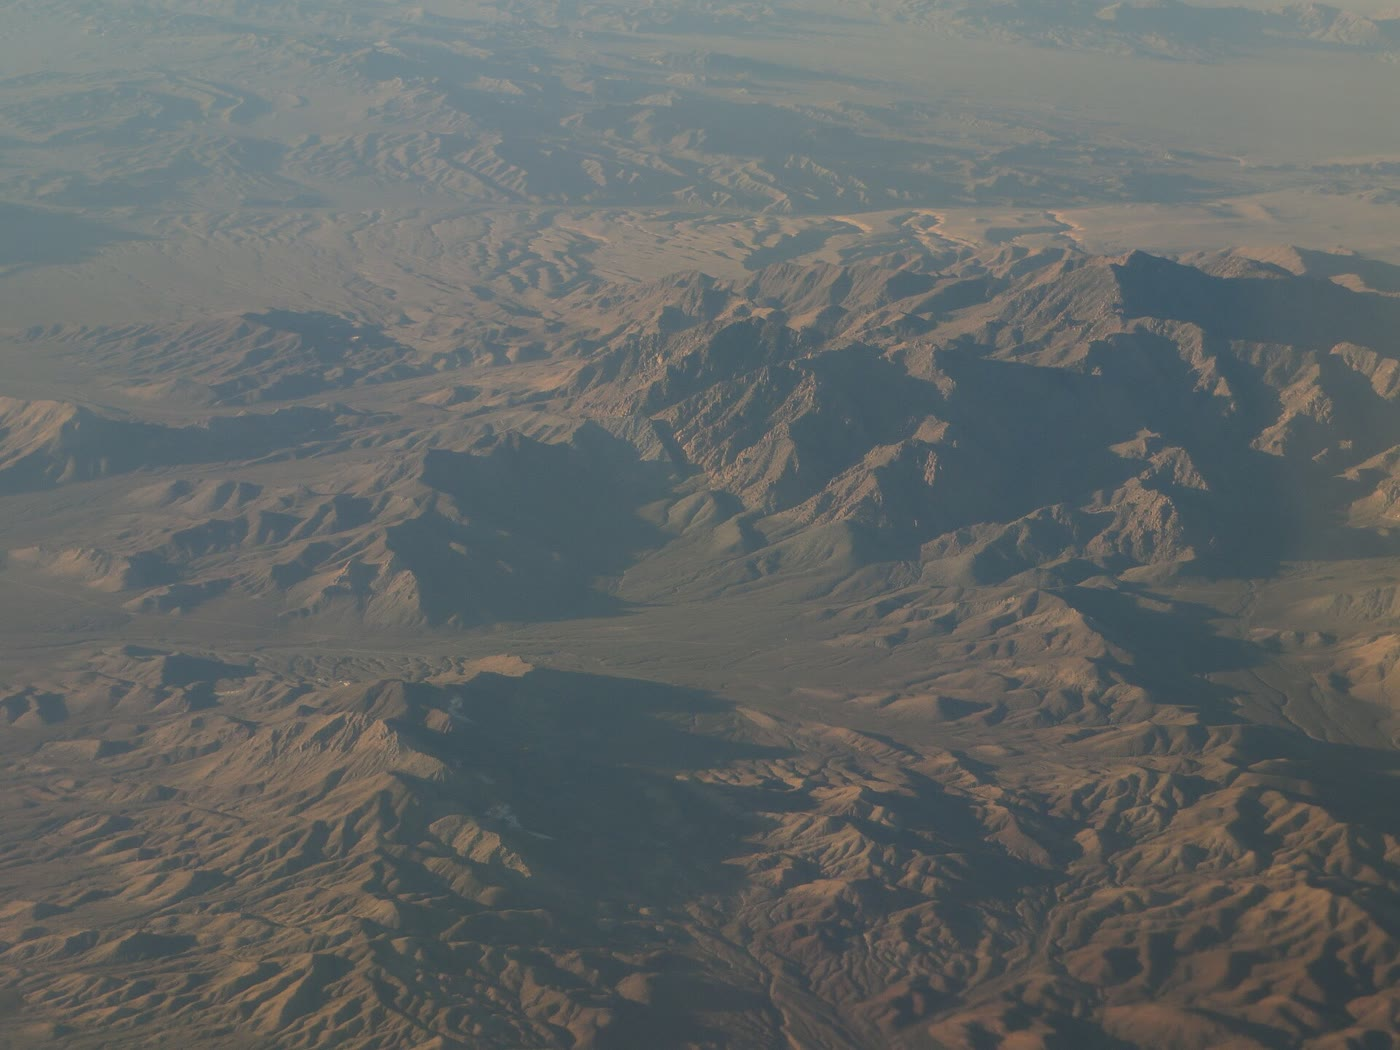
\includegraphics[width=\linewidth]{images/book5/b3-basin-and-range.jpg}

{\scriptsize कैलिफ़ोर्निया में डेथ वैली के दक्षिण में, ऊपर से देखी गई बेसिन-एंड-रेंज स्थलाकृति,
झुके भ्रंश-खंडों की समांतर श्रेणियाँ, जो
अवसाद से भरी द्रोणियों से अलग होती हैं। फ़ोटो Ken Lund, CC BY-SA 2.0.}
\end{minipage}
\end{inthefield}
% ledger: photo:b3-basin-and-range

\section{अभ्यास}

\begin{exercise}[$\star$]\label{exo:b3:extension-strike-slip:1}
कठोर डोमिनो-खंडों के एक क्षेत्र के भ्रंशों की नति \ang{35} है; ये
\ang{50} पर बने। संस्तरों की नति और प्रसार गुणक परिकलित कीजिए।
\end{exercise}

\begin{exercise}[$\star$]\label{exo:b3:extension-strike-slip:2}
बताइए कि प्रत्येक सोपान द्रोणी खोलता है या कटक उठाता है: दाएँ-पार्श्वीय भ्रंश, दाईं ओर
सोपान; दाएँ-पार्श्वीय भ्रंश, बाईं ओर सोपान; बाएँ-पार्श्वीय भ्रंश, बाईं ओर
सोपान; बाएँ-पार्श्वीय भ्रंश, दाईं ओर सोपान।
\end{exercise}

\begin{exercise}[$\star$]\label{exo:b3:extension-strike-slip:3}
मृत सागर रूपांतर भ्रंश लगभग \qty{20}{Myr} में \qty{105}{km} खिसका है।
\unit{mm/yr} में माध्य दर परिकलित कीजिए और उसकी तुलना उस \qty{6}{mm/yr} से कीजिए
जो मृत सागर द्रोणी के लिए प्रयुक्त हुई थी।
\end{exercise}

\begin{exercise}[$\star$]\label{exo:b3:extension-strike-slip:4}
बेसिन-एंड-रेंज के केंद्रीय भाग में \qty{235}{km} का प्रसार
\qty{200}{\percent} के बराबर है। प्रसार से पहले और बाद में क्षेत्र की चौड़ाई परिकलित कीजिए। वही
कार्य उत्तरी भाग के लिए, \qty{50}{\percent} पर, कीजिए।
\end{exercise}

\begin{exercise}[$\star\star$]\label{exo:b3:extension-strike-slip:5}
सैन एंड्रियास भ्रंश कम से कम \qty{563}{km} खिसका है, 15 से
\qty{20}{Myr} में। माध्य दरों का परास परिकलित कीजिए, और उनकी तुलना
लगभग \qty{51}{mm/yr} के वर्तमान विस्थापन से कीजिए। इस अंतर की व्याख्या क्या कर सकता है?
\end{exercise}

\begin{exercise}[$\star\star$]\label{exo:b3:extension-strike-slip:6}
$\mu = 0.6$ मानकर, वह अनुपात $\sigma_1/\sigma_3$ परिकलित कीजिए जो सामान्य भ्रंशों को
फिसलाने के लिए आवश्यक है, जिनकी नति \ang{60}, \ang{50} और \ang{40} है, तथा लॉक-अप नति भी।
\end{exercise}

\begin{exercise}[$\star\star$]\label{exo:b3:extension-strike-slip:7}
$\mu = 0.4$ और $\mu = 0.2$ के लिए सामान्य भ्रंश की लॉक-अप नति परिकलित कीजिए।
\ang{15} नति वाला भ्रंश किस घर्षण गुणांक पर
ऊर्ध्वाधर $\sigma_1$ के अंतर्गत फिसल सकेगा?
\end{exercise}

\begin{exercise}[$\star\star$]\label{exo:b3:extension-strike-slip:8}
स्लिप के समांतर भूकंपीय परिच्छेद पर, एक \omterm{def:b3:extension-strike-slip:detachment}{लिस्ट्रिक भ्रंश} का क्षैतिज विस्थापन
\qty{2.5}{km} है; यह \qty{4.0}{km} गहराई पर एक विलगन में समतल हो जाता है। परिकलित
कीजिए: मूल ऊपरी भित्ति के शीर्ष के नीचे के अवनमन का क्षेत्रफल, और
पहले \qty{1.5}{km} गहरे संस्तर के नीचे का।
\end{exercise}

\begin{exercise}[$\star\star$]\label{exo:b3:extension-strike-slip:9}
मृत सागर द्रोणी \qty{132}{km} लंबी है और
अपने अक्ष के अनुदिश 1.19 गुणक से खिंची हुई है। इसकी आरंभिक लंबाई और खिंचाव,
तथा \qty{6}{mm/yr} की दर पर उस खिंचाव में लगने वाला समय परिकलित कीजिए।
\end{exercise}

\begin{exercise}[$\star\star\star$]\label{exo:b3:extension-strike-slip:10}
उनके भ्रंशों के लंबवत मापे गए \qty{3.0}{km} दूरी पर स्थित खंड
\ang{60} की भ्रंश-नति से \ang{45} की ओर घूमते हैं। घूमने से पहले और बाद में एक खंड की
क्षैतिज चौड़ाई, प्रति खंड प्रसार, और संस्तरों की नति परिकलित कीजिए।
संस्तर भ्रंशों से विपरीत दिशा में क्यों नत होने चाहिए?
\end{exercise}

\begin{exercise}[$\star\star\star$]\label{exo:b3:extension-strike-slip:11}
R और R$'$ अपरूपणों तथा तनाव दरारों के कोण,
जिसका $\phi = \ang{40}$ है, बाएँ-पार्श्वीय क्षेत्र में पूर्व--पश्चिम स्ट्राइक वाली चट्टान के लिए,
दिगंश के रूप में, और उनकी विस्थापन दिशाएँ ज्ञात कीजिए।
\end{exercise}

\begin{exercise}[$\star\star\star$]\label{exo:b3:extension-strike-slip:12}
\omterm{def:b3:extension-strike-slip:domino}{डोमिनो भ्रंशन} वाला एक क्षेत्र बनता है, जिसके भ्रंश फिसलने की सर्वोत्तम नति पर बनते हैं, और
तब तक घूमता है जब तक वे लॉक-अप नहीं हो जाते। घूर्णन अकेले से मिलने वाला सबसे बड़ा प्रसार गुणक
$\mu = 0.6$ और $\mu = 0.85$ के लिए परिकलित कीजिए, और यह भी
बताइए कि नए भ्रंश बनने से पहले किन चट्टानों को और खींचा जा सकता है।
\end{exercise}

\section{समस्या: मेरो अर्ध-ग्राबेन}

\begin{problem}[{सप्ताहांत समस्या --- एक काल्पनिक दरार-सीमा का प्रसार,
उसके डोमिनो, लिस्ट्रिक भ्रंश, कायांतरी क्रोड संकुल और
स्थानांतरण भ्रंश से}]
\label{pb:b3:extension-strike-slip:1}
% values: calc/ch09.py; domino_extension.py; rollover.py
मेरो अर्ध-ग्राबेन एक काल्पनिक द्रोणी है, जो महाद्वीपीय
दरार की सीमा पर स्थित है। इसका मुख्य भ्रंश लिस्ट्रिक है, सतह पर इसकी नति \ang{60} है। इसकी
ऊपरी भित्ति में \qty{24.0}{km} चौड़ा एक क्षेत्र समतल भ्रंशों द्वारा कटा है, जिनकी अब नति
\ang{42} पूर्व की ओर है, जिनके बीच संस्तर \ang{18} पश्चिम की ओर नत हैं। भूकंपीय परिच्छेद पर
स्लिप के समांतर, मुख्य भ्रंश का क्षैतिज विस्थापन \qty{3.2}{km} है, और उसकी ऊपरी भित्ति का शीर्ष
अपने मूल स्तर से नीचे धँसा हुआ है, जिसका क्षेत्रफल
\qty{16.0}{km^2} है। स्ट्राइक के अनुदिश दक्षिण की ओर अपरदन ने उसी तंत्र की ऊपरी
प्लेट हटा दी और \omterm{def:b3:extension-strike-slip:core-complex}{कायांतरी क्रोड संकुल} उजागर किया है। उत्तर की ओर एक
बाएँ-पार्श्वीय स्थानांतरण भ्रंश इस अर्ध-ग्राबेन को अगले से जोड़ता है। मान लीजिए $\mu =
0.6$, $g = \qty{9.8}{m/s^2}$ तथा भूपर्पटी का घनत्व
\qty{2800}{kg/m^3} है।

\medskip\noindent\textbf{भाग I --- डोमिनो।}
\begin{enumerate}
  \item भ्रंशों की आरंभिक नति वर्तमान भ्रंश
        और संस्तर नतियों का योग क्यों है? उसे ज्ञात कीजिए, और उसकी तुलना एंडरसन के सिद्धांत से कीजिए।
  \item क्षेत्र का प्रसार गुणक परिकलित कीजिए।
  \item इसकी आरंभिक चौड़ाई और वह प्रसार परिकलित कीजिए जिसे यह अभिलिखित करता है।
  \item भ्रंशों को अभी फिसलाने के लिए आवश्यक \omterm{def:b3:structural-analysis:palaeostress}{प्रतिबल अनुपात} $\sigma_1/\sigma_3$ परिकलित कीजिए,
        और उसकी तुलना नए, उपयुक्त अभिविन्यास वाले भ्रंशों के अनुपात से कीजिए।
  \item ये भ्रंश किस नति पर लॉक-अप होते हैं, और केवल घूर्णन से क्षेत्र कितना प्रसार गुणक
        प्राप्त कर सकता है? तब क्या होता है?
\end{enumerate}

\medskip\noindent\textbf{भाग II --- लिस्ट्रिक मुख्य भ्रंश।}
\begin{enumerate}[resume]
  \item स्थिर-क्षैतिज विस्थापन रचना की सहायता से ऊपरी भित्ति के
        संस्तर भ्रंश की ओर क्यों झुकते हैं, यह समझाइए।
  \item विलगन की गहराई परिकलित कीजिए।
  \item अवनमन क्षेत्रफल \qty{10}{\percent} की सीमा तक ज्ञात है। गहराई कितनी सटीकता से
        ज्ञात है?
  \item जो संस्तर पहले \qty{2.0}{km} गहराई पर था, उसके लिए आप कौन सा अवनमन क्षेत्रफल
        पूर्वानुमानित करते हैं?
  \item मुख्य भ्रंश के आर-पार क्षैतिज प्रसार कितना है?
  \item अर्ध-ग्राबेन के अवसाद भ्रंश की सक्रियता को
        कैसे अभिलिखित करते हैं?
\end{enumerate}

\medskip\noindent\textbf{भाग III --- कायांतरी क्रोड संकुल।}
\begin{enumerate}[resume]
  \item निचली भित्ति के मायलोनाइट \qty{5.5}{kbar} पर साम्यावस्था में पहुँचे थे। उनकी
        गहराई परिकलित कीजिए।
  \item उनके अभ्रक \qty{24}{Ma} पर ऑर्गन के लिए बंद हो गए, और उन्हीं मायलोनाइटों के कंकड़
        अर्ध-ग्राबेन के भराव में \qty{16}{Ma} पर दिखाई देते हैं। माध्य उत्खनन-दर परिकलित कीजिए,
        बंद होने की गहराई को
        पिछले प्रश्न की गहराई मानते हुए।
  \item मायलोनाइटों को ऊपर लाने के लिए विलगन पर कितना स्लिप चाहिए,
        जिसकी माध्य नति \ang{30} है, और कितना क्षैतिज प्रसार चाहिए?
  \item आज सतह पर विलगन की नति \ang{15} है। क्या यह उस नति पर
        ऊर्ध्वाधर $\sigma_1$ के अंतर्गत फिसल सकता था? बचने के दो उपाय बताइए।
  \item यदि यह गहराई पर \ang{45} पर फिसला था, तो उजागर भाग किस कोण से
        घूम गया है, और क्यों?
  \item \omterm{def:b3:extension-strike-slip:core-complex}{कायांतरी क्रोड संकुल} के प्रसार की तुलना
        अर्ध-ग्राबेन के प्रसार से कीजिए।
\end{enumerate}

\medskip\noindent\textbf{भाग IV --- स्थानांतरण भ्रंश।}
\begin{enumerate}[resume]
  \item बाएँ-पार्श्वीय स्थानांतरण भ्रंश \qty{4.0}{km} बाईं ओर सोपानित होता है, और उसकी दो शाखाएँ
        \qty{3.0}{km} तक परस्पर अतिव्याप्त हैं। क्या यह सोपान एक द्रोणी खोलता है
        या एक कटक उठाता है?
  \item यह भ्रंश \qty{5}{mm/yr} की दर से \qty{1.2}{Myr} तक फिसला है। विस्थापन
        परिकलित कीजिए।
  \item खुला क्षेत्रफल, द्रोणी-तल की लंबाई (अतिव्याप्ति और विस्थापन का
        योग) और उसका लंबाई और चौड़ाई का अनुपात परिकलित कीजिए।
  \item इस अनुपात की तुलना मृत सागर द्रोणी के अनुपात से कीजिए। वह द्रोणी
        \qty{132}{km} लंबी और 7 से \qty{10}{km} चौड़ी है।
  \item जहाँ वही भ्रंश दूसरी दिशा में मुड़ता है, वहाँ कौन सी संरचना बनती है, और
        उसके आर-पार का अनुप्रस्थ काट क्या दिखाएगा?
  \item मेरो अर्ध-ग्राबेन के आर-पार कुल क्षैतिज प्रसार क्या है,
        जो उसके मुख्य भ्रंश और डोमिनो से बना है?
\end{enumerate}
\end{problem}
